% Working draft of the IJHMT version of the LESTO iodine methods paper, in
% the arxiv.sty layout of ../main.tex with line numbers.  Same content as the
% Elsevier wrapper lesto-ijhmt-elsarticle.tex: the IJHMT title, the shared
% journal abstract and data statement (../sections/*-journal.tex), keywords,
% nomenclature.tex, the shared sections and declarations.tex.
% Build with ./build.sh in this folder.
\documentclass{article}
% Shared files are found relative to the manuscript root: ../arxiv.sty,
% and the generated/... inputs of the section files.
\makeatletter
\def\input@path{{../}}
\makeatother
\usepackage{arxiv}
\usepackage{iftex}
\ifPDFTeX\usepackage[utf8]{inputenc}\fi
\usepackage[T1]{fontenc}
\usepackage{amsmath,amssymb,booktabs,graphicx,microtype,xcolor}
\usepackage[version=4]{mhchem}
\usepackage[numbers,sort&compress]{natbib}
\usepackage{url}
\usepackage{hyperref}
\usepackage{cleveref}
\usepackage{authblk}
\usepackage{lineno}
% lineno skips the lines around amsmath displays; the usual patch numbers the
% paragraph lines before and after each display environment again.
\newcommand*\patchAmsMathEnvironmentForLineno[1]{%
  \expandafter\let\csname old#1\expandafter\endcsname\csname #1\endcsname
  \expandafter\let\csname oldend#1\expandafter\endcsname\csname end#1\endcsname
  \renewenvironment{#1}%
    {\linenomath\csname old#1\endcsname}%
    {\csname oldend#1\endcsname\endlinenomath}}%
\newcommand*\patchBothAmsMathEnvironmentsForLineno[1]{%
  \patchAmsMathEnvironmentForLineno{#1}%
  \patchAmsMathEnvironmentForLineno{#1*}}%
\AtBeginDocument{%
  \patchBothAmsMathEnvironmentsForLineno{equation}%
  \patchBothAmsMathEnvironmentsForLineno{align}%
  \patchBothAmsMathEnvironmentsForLineno{gather}%
  \patchBothAmsMathEnvironmentsForLineno{multline}}
% Shared sections use table* for wide tables (needed in two-column layouts);
% give table* the same caption spacing that arxiv.sty gives table.
\makeatletter
\renewenvironment{table*}
  {\setlength{\abovecaptionskip}{\@belowcaptionskip}%
   \setlength{\belowcaptionskip}{\@abovecaptionskip}%
   \@dblfloat{table}}
  {\end@dblfloat}
\makeatother
\graphicspath{{../figures/}}
\setlength{\emergencystretch}{1.5em}
% Generated from saved completed reports.
\newcommand{\BaselineCases}{15}
\newcommand{\FollowupCases}{64}
\newcommand{\ProductionCases}{19}
\newcommand{\TimeMin}{0.0043}
\newcommand{\TimeMax}{0.323}
\newcommand{\MeshMin}{2.06}
\newcommand{\MeshMax}{10.58}
\newcommand{\ProductionResidue}{1.41\times10^{-12}}
\newcommand{\SteelLLOne}{15.35}
\newcommand{\SteelLLTwo}{8.95}
\newcommand{\SteelLLThree}{1.98}
\newcommand{\SteelUpOne}{10.47}
\newcommand{\SteelUpTwo}{10.58}
\newcommand{\SteelUpThree}{2.13}
\newcommand{\PureLLOne}{5.70}
\newcommand{\PureLLTwo}{2.15}
\newcommand{\PureUpOne}{6.57}
\newcommand{\PureUpTwo}{5.06}
\newcommand{\SteelOrderOne}{1.3}
\newcommand{\SteelOrderTwo}{3.7}
\newcommand{\SteelErrApparent}{2.5}
\newcommand{\SteelErrSecond}{3.6}
\newcommand{\SteelSmoothThree}{0.67}
\newcommand{\SteelTotalThree}{0.015}
\newcommand{\SteelCentroidRange}{0.6}
\newcommand{\SteelCentroidTRange}{0.9}
\newcommand{\UpLLOne}{20.8}
\newcommand{\UpLLTwo}{14.1}
\newcommand{\UpLLThree}{11.3}
\newcommand{\UpLLFour}{7.7}
\newcommand{\PureUpLLMin}{9.0}
\newcommand{\PureUpLLMax}{13.2}
\newcommand{\VLSteelMax}{2.8}
\newcommand{\VLPureMax}{1.8}
\newcommand{\VLSteelThree}{1.16}
\newcommand{\VLPureThree}{0.27}
\newcommand{\IterPure}{1.09\times10^{-13}}
\newcommand{\IterSteelLow}{4.89\times10^{-13}}
\newcommand{\IterSteelHigh}{0.021}
\newcommand{\LobRMS}{18}
\newcommand{\LobRMSTemp}{35}
\newcommand{\LobRMSVap}{35}
\newcommand{\LobRMSGas}{17}
\newcommand{\LobCoarse}{0.2}
\newcommand{\LobDigitised}{1.0}
\newcommand{\LobFiveInlet}{548}
\newcommand{\LobFiveGas}{+3}
\newcommand{\LobFiveGasFraction}{4.0}
\newcommand{\LobLOneMin}{0.37}
\newcommand{\LobLOneMax}{0.89}
\newcommand{\LobRMSInlet}{135}
\newcommand{\LobFiveMain}{836}
\newcommand{\LobSixDeposit}{98.1}
\newcommand{\LobFiveUpstream}{1.2}
\newcommand{\LobShiftMin}{1}
\newcommand{\LobShiftMax}{4}
\newcommand{\LobCellsProd}{22{,}896}
\newcommand{\LobCellsCoarse}{10{,}176}
\newcommand{\GraetzBound}{1.69\times10^{-12}}
\newcommand{\GraetzRuns}{45}
\newcommand{\GraetzCriteria}{27}
\newcommand{\GraetzOrderHalfMin}{1.99}
\newcommand{\GraetzOrderHalfMax}{2.00}
\newcommand{\GraetzOrderNoneMin}{1.004}
\newcommand{\GraetzOrderNoneMax}{1.008}
\newcommand{\GraetzOrderSBHalf}{2.00--2.01}
\newcommand{\GraetzOrderSBNone}{1.01--1.02}
\newcommand{\GraetzGCIHalfMax}{1.89\times10^{-4}}
\newcommand{\GraetzGCINoneMin}{0.155}
\newcommand{\GraetzGCINoneMax}{0.341}
\newcommand{\GraetzExtHalfMax}{9.47\times10^{-9}}
\newcommand{\GraetzExtNoneMax}{1.10\times10^{-5}}
\newcommand{\GraetzMuH}{7.09\times10^{-9}}
\newcommand{\LobDiffA}{+26}
\newcommand{\LobDiffB}{+19}
\newcommand{\LobDiffC}{+16}
\newcommand{\LobDiffD}{$-$11}
\newcommand{\LobDiffE}{$-$14}

\newcommand{\vect}[1]{\mathbf{#1}}
\newcommand{\units}[1]{\,\mathrm{#1}}
% Clearly visible placeholder for information only the authors can supply.
\newcommand{\confirm}[1]{\textcolor{red}{[AUTHOR TO CONFIRM: #1]}}
\title{Competition between radial diffusion and interfacial exchange in
thermal-gradient deposition columns: conservative modeling of iodine
transport}
\renewcommand\Authfont{\bfseries}
\setlength{\affilsep}{0em}
\author[1]{Jan Kren\thanks{Corresponding author:
  \confirm{corresponding e-mail}}}
\author[1]{Bojan Ni\v{c}eno}
\affil[1]{Paul Scherrer Institute, 5232 Villigen PSI, Switzerland}
\date{\today}
\renewcommand{\shorttitle}{Radial diffusion and interfacial exchange in
  deposition columns}
\renewcommand{\headeright}{Draft for IJHMT}
\renewcommand{\undertitle}{Draft for the International Journal of Heat and
  Mass Transfer}
\hypersetup{colorlinks=true,linkcolor=blue,citecolor=blue,urlcolor=blue,
  pdftitle={Competition between radial diffusion and interfacial exchange
    in thermal-gradient deposition columns},
  pdfauthor={Jan Kren and Bojan Niceno}}

\begin{document}
\raggedbottom
\maketitle
\begin{abstract}
% Journal abstract (<= 250 words), shared by pof/lesto-pof.tex and
% ijhmt/lesto-ijhmt.tex.  Recount after any edit.
We present an OpenFOAM finite-volume model of vapour transport in
laminar thermal-gradient columns: nine Pb--Bi--I gases in a frozen
helium carrier, with element-conserving gas equilibrium and shared wall
inventories.
Reversible iodide exchange follows a Hertz--Knudsen--Schrage law in
series with the near-wall diffusive resistance; on a Graetz--Robin
problem this face flux converges at second order, a cell-centre sink at
first order. In 79 simulations the largest raw element-balance
residue is $1.41\times10^{-12}$ of supplied material.
Halving the time step or adding correctors changes iodine profiles by
at most 0.323\%. First-order upwind advection differs from
a bounded limited-linear scheme by up to 20.8\% at equal mesh.
Refining from 41,472 to 93,312 cells changes profiles by
\SteelUpThree--\UpFourOthersMax\% (upwind, four cases) and 1.98\%
(bounded, one case), with inconsistent observed orders. A wall
Damk\"ohler sweep reproduces the kinetic and diffusion
limits and shows that radial diffusion, not interfacial
kinetics, limits wall exchange in the production cases; with the
bounded scheme, accommodation changes alter iodine profiles by at most
\PSAlphaTwoMax\%, diffusivity changes by up to \PSDMax\%.
A $+29\units{kJ\,mol^{-1}}$ shift in the BiI gas Gibbs energy changes
the BiI$_3$ share of deposited iodide iodine from 94.58\% to 2.01\%. Without tuning, the wall
law gives deposition-onset temperatures of five PbI$_2$ experiments
with an RMS deviation of 18 K, against 35 K for two published models;
because carrier, vapour-pressure and source assumptions differ and
computed peaks lie 1--4 cm upstream, this promising result does not yet
isolate the wall treatment. The results support a conservative method,
not independent predictive validation.

\end{abstract}
\keywords{Thermal-gradient tube flow \and Vapor deposition \and
Hertz--Knudsen--Schrage \and Laminar mass transfer \and Wall
Damk\"ohler number \and Finite-volume method \and Numerical verification}

\linenumbers

% IJHMT nomenclature, shared by lesto-ijhmt.tex (arxiv.sty draft) and
% lesto-ijhmt-elsarticle.tex.
% Nomenclature list: symbol column 8.5em, group headings in bold.
\newenvironment{longnomenclature}
  {\begin{list}{}{\setlength{\labelwidth}{8em}\setlength{\leftmargin}{8.5em}%
    \setlength{\labelsep}{0.5em}\setlength{\itemsep}{0pt}%
    \setlength{\parsep}{0pt}\renewcommand{\makelabel}[1]{##1\hfil}}}
  {\end{list}}
\newcommand{\nomgroup}[1]{\item[\textbf{#1}]\mbox{}}

\section*{Nomenclature}
\label{sec:nomenclature}
{\small
\begin{longnomenclature}
\nomgroup{Latin symbols}
\item[$A_f$] wall face area, m$^2$
\item[$a_{\rm Pb}$, $a_{\rm Bi}$] activities of Pb and Bi in LBE
\item[$b_k$] concentration of element $k$, mol\,m$^{-3}$
\item[$C_e$, $s_i$] multipliers of the HKS conductance
\item[$c$, $\bar c$, $c_{\rm eq}$] vapour concentration, its cross-section
  mean and its equilibrium value (channel), mol\,m$^{-3}$
\item[$D_i$] molecular diffusivity of gas $i$, m$^2$\,s$^{-1}$
\item[$d$] tube diameter, m
\item[$d_f$] distance from cell centre to wall face, m
\item[$G_i$] HKS conductance, s\,m$^{-1}$
\item[$G_{i,f}^{\rm eff}$] effective (kinetic and half-cell diffusion)
  conductance, s\,m$^{-1}$
\item[$G^\circ$] standard Gibbs energy, J\,mol$^{-1}$
\item[$h$] channel half-height, m
\item[$J$] wall molar flux in the channel, mol\,m$^{-2}$\,s$^{-1}$
\item[$j_i$] wall mass flux, positive from condensate to gas,
  kg\,m$^{-2}$\,s$^{-1}$
\item[$K_{f,i}$] formation equilibrium constant of gas $i$
\item[$K_r$] equilibrium constant of the BiI reaction
\item[$k_w$] first-order wall uptake velocity, m\,s$^{-1}$
\item[$M_i$] molar mass, kg\,mol$^{-1}$
\item[$m_i$] source mass of compound $i$, kg
\item[$\dot m$] helium mass flow, kg\,s$^{-1}$
\item[$N_k$] molar inventory of element $k$, mol
\item[$N_r$] number of radial cells
\item[$p$] pressure, Pa
\item[$p_i$] partial pressure of gas $i$, Pa
\item[$p_{{\rm eq},i}$] equilibrium pressure over the condensate, Pa
\item[$p^\circ$] standard pressure, $10^5$\,Pa
\item[$p_h$] source pressure, Pa
\item[$q_{1,i}$, $q_{2,k}$] source rates of models Q1 and Q2,
  mol\,s$^{-1}$
\item[$q_{\rm He}$] helium molar flow, mol\,s$^{-1}$
\item[$R$] gas constant, J\,mol$^{-1}$\,K$^{-1}$; tube radius, m
\item[$R_k$] balance residue of element $k$, mol
\item[$r$, $x$] radial and axial coordinates, m
\item[$S_i^{\rm rel}$, $S_i^{\rm wall}$] release and wall sources,
  kg\,m$^{-3}$\,s$^{-1}$
\item[$T$] temperature, K
\item[$T_h$] source-furnace temperature, K
\item[$t$] time, s
\item[$U_b$] bulk velocity, m\,s$^{-1}$
\item[$\vect{u}$] carrier velocity, m\,s$^{-1}$
\item[$Y_i$] mass of gas $i$ per unit carrier mass
\nomgroup{Greek symbols}
\item[$\alpha_i$] accommodation coefficient
\item[$\beta$] metal saturation of source model Q2
\item[$\lambda_k$] dimensionless element potential
\item[$\mu$] dynamic viscosity, Pa\,s (\cref{sec:regime}); decay rate,
  m$^{-1}$ (\cref{sec:verification})
\item[$\nu_{ki}$] atoms of element $k$ in gas $i$
\item[$\rho$] carrier density, kg\,m$^{-3}$
\item[$\tau_{\rm exp}$] duration of the experiment, s
\item[$\chi_i$] $\rho RT/M_i$, Pa
\nomgroup{Dimensionless numbers}
\item[Bi] Biot number, $k_wR/D$
\item[$\mathrm{Da}_i$] wall Damk\"ohler number, \cref{eq:damkohler}
\item[Gr] Grashof number
\item[$\hat J$] normalised wall flux, $Jh/[D(\bar c-c_{\rm eq})]$
\item[Pe] P\'eclet number: $\mathrm{Re\,Sc}$ (diameter based,
  \cref{sec:regime}); $U_bR/D$ (Graetz problem, \cref{sec:verification})
\item[Re] Reynolds number, $4\dot m/(\pi d\mu)$
\item[Sc] Schmidt number
\nomgroup{Subscripts}
\item[$c$] cell centre
\item[$f$] wall face
\item[$i$] gas species
\item[$k$] element (Pb, Bi, I)
\item[$w$] wall
\end{longnomenclature}
}


\section{Introduction}
\label{sec:intro}
Iodine released from lead--bismuth eutectic (LBE) can travel in several
chemical forms before it deposits on cooler surfaces. The chemical form
matters because it sets both the gas-phase inventory available for
transport and the equilibrium pressure that governs wall exchange.
Liu et al.\ \cite{Liu2025chemical} studied this behaviour by evaporating
pure iodides and iodine-containing LBE into helium, separating the
products along a negative temperature gradient and characterising the
deposits. Their measurements give spatially resolved evidence for
PbI$_2$ and BiI$_3$ deposition, and for potassium-containing deposits in
some LBE experiments. Linking such measurements to a transport
calculation needs more than a single deposition temperature: the
temperature-coordinate mapping, the carrier flow, the source history
and the gas composition all affect the predicted distribution.

Seen as a fluid-dynamics problem, a thermal-gradient column is a slow
laminar flow of an inert carrier through a long, narrow tube whose wall
temperature falls by several hundred kelvin along its length
(\cref{fig:temperature}). Trace vapours released near the hot end are
advected downstream by a carrier whose density and velocity vary with
the imposed temperature, and they diffuse radially towards the wall.
Where the local vapour pressure exceeds the equilibrium pressure at the
wall temperature, material is lost to the wall; where it falls below
that pressure, existing deposits can evaporate again. The deposition
profile is therefore set by the competition between axial advection,
radial diffusion to the wall and the interfacial exchange law. This is
a Graetz-type wall mass-transfer problem \cite{Shah1978circular}, but
with a nonlinear wall condition that depends on the local wall
temperature and condensed inventory. The same coupling underlies the
interpretation of thermochromatographic experiments
\cite{Eichler1975verfluchtigung,Zvara1985simulation,Zvara2008inorganic}.

Lobresco et al.\ \cite{Lobresco2026assessment} compared temperature-based
and vapour-pressure-driven CFD deposition models. Temperature-based
models require a calibrated deposition law; vapour-pressure-driven
models link deposition to vapour-pressure data through interfacial
kinetics. Their study also motivates extending transport models to
multiple chemical species and to thermodynamic equilibrium. A
multispecies model adds a consistency requirement. Changes in chemical
form must conserve the transported elements, and different gas pathways
that lead to the same condensed material must share one physical wall
inventory. Even an internally consistent implementation can give
uncertain experimental predictions if its thermodynamic or source
inputs are poorly constrained.

We address these issues in the finite-volume framework of OpenFOAM
\cite{Weller1998tensorial}. The model transports nine Pb--Bi--I gases in
a prescribed helium carrier. Homogeneous gas equilibrium redistributes
the local elemental inventory, and separate interfacial channels
exchange material with immobile condensed wall inventories. The wall
flux combines interfacial kinetic conductance with diffusion over the
distance from the neighbouring cell centre to the wall. This avoids
representing deposition through an arbitrarily chosen volumetric
wall-layer thickness. It does not remove spatial discretisation error.

General thermodynamic packages such as GEM-Selektor and its GEMS3K
kernel \cite{Kulik2013gemselektor} also support equilibrium-based
reactive transport. The software developed here has a GEMS3K interface,
but the calculations reported in this paper use a specialised ideal-gas
element-potential solver with tabulated formation constants. We
therefore distinguish the thermodynamic formulation from the numerical
engine used for the reported simulations. Condensed phases enter
through wall exchange, not through homogeneous cell equilibrium.

All experimental input comes from the published paper. No
author-supplied temperature files, release histories or
mass-flow-controller reference conditions are available. We therefore
do not infer a unique physical source from the deposition data.
Instead, we report the consequences of two explicit source models and
of selected variations in flow, diffusion, interfacial accommodation
and thermodynamic data. Separate time-step and mesh studies show which
conclusions survive numerical refinement. We treat a
temperature-coordinate discrepancy in the silica experiment as an
input-consistency problem: alternative mappings are defined from
published quantities before the resulting CFD profiles are compared.

The contribution is a documented, conservative coupling of transport,
gas equilibrium and wall exchange, together with a completed numerical
and input-sensitivity assessment. The evidence comprises 15 baseline
and 64 follow-up simulations of the three available experimental
configurations. These are computational cases, not independent
experimental replicates. The scope is deliberately limited to the
executed model: a fixed carrier and temperature field, prescribed
release, ideal-gas speciation, and wall deposits without aerosol
formation or surface-material-specific chemistry. Comparisons with
experiment are conditional assessments of this model, not a claim of
independent predictive validation.

\section{Experimental basis and input reconstruction}
\label{sec:experiments}
\subsection{Available configurations}
Liu et al.\ \cite{Liu2025chemical} used 1.25 m columns with an inner
diameter of 4.8 mm for 316L stainless steel and 5.0 mm for fused
silica. A 15 mm sample boat was inserted into a hot starting furnace,
followed by a second furnace that imposed a decreasing temperature
profile. Helium carried the evaporated material downstream. After
three hours the source was withdrawn, the furnaces and gas flow were
turned off, and the column cooled before the deposits were analysed.
Temperature measurements and radiotracer scans used 1 cm increments.

\Cref{tab:experiments} lists the three configurations for which both
temperature curves and iodine scans could be reconstructed. The
stand-alone BiI$_3$ experiment at 800\,$^\circ$C was not run, because
its axial temperature profile is not published; it is neither given a
surrogate profile nor counted as an unsuccessful simulation.
\begin{table*}[tb]
\centering
\caption{Published configurations used in the baseline matrix. Sample
masses are initial masses, not the amounts released in a 60 s run.
Every experimental evaporation period was 10,800 s.}
\label{tab:experiments}
\begin{tabular}{llrrr}
\toprule
Identifier & Column & Diameter (mm) & Sample (mg) & He (mL/min) \\
\midrule
PbI2\_SS & Steel & 4.8 & 14.6 & 100 \\
LBE-I\_SS\_II & Steel & 4.8 & 346.0 & 45 \\
LBE-I\_SiO2\_I & Silica & 5.0 & 368.3 & 45 \\
\bottomrule
\end{tabular}
\end{table*}

Both LBE samples had a reported iodine mole fraction of
$9.04\times10^{-4}$ and a 900\,$^\circ$C starting furnace. Their
reported deposited iodine amounts were 0.191 and 0.203 mg,
respectively. These amounts set the prescribed mean iodine source in
the present cases; they are not measurements of a time-resolved
evaporation rate or of inlet speciation.

\subsection{Digitisation and coordinate assumptions}
We digitized the axial temperature curves and iodine histograms from
the published figures. Temperatures are interpolated linearly to cell
centers and wall faces; beyond the plotted interval they are held at
the nearest endpoint value. The computational coordinate is the plotted
coordinate, whose origin relative to the physical boat and furnace is
unconfirmed (\cref{fig:temperature}); the silica-coordinate study
varies this assumption.

The recorded digitisation resolutions are approximately 1 mm in
position, 4 K in temperature and 0.4 percentage points in histogram
height. They describe raster extraction only, not coordinate registration,
detector response, temperature reproducibility or calibration, and the
uncertainties printed with the deposition temperatures are not
uncertainties of every profile bin. The reconstructed histograms sum to 99.17\%, 96.70\% and
102.24\% for pure PbI$_2$, steel LBE and silica LBE. The primary
comparison keeps these sums and does not silently renormalise them.

In the LBE scans, the paper assigns 6.6\% and 7.0\% of the iodine to
KI, which lies outside the Pb--Bi--I species set. We scale the model
profile to the remaining 93.4\% or 93.0\%, while the measured histogram
keeps all its published deposits. A second, explicitly conditional
comparison normalises both profiles over their common scanned range
(\cref{sec:comparison}). Neither comparison supplies the omitted
potassium chemistry.

\begin{figure*}[tb]
\centering
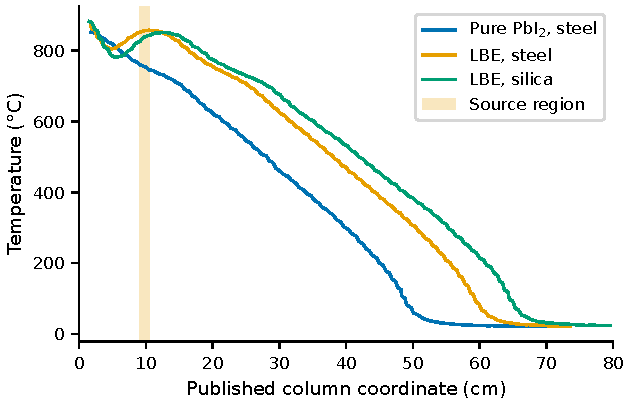
\includegraphics{temperature_profiles.pdf}
\caption{Axial temperature curves digitized from Liu et al.\
\cite{Liu2025chemical} for the three configurations, with the assumed
computational source interval. Beyond the plotted range, the CFD domain
holds the endpoint values constant. The curves reconstruct published
figures; they are not temperature fields predicted by a conjugate
heat-transfer calculation.}
\label{fig:temperature}
\end{figure*}

\subsection{Simulation duration and measurement protocol}
All source-driven cases run for 60 s with a source rate based on the
10,800 s experimental period, so they release $1/180$ of the assumed
three-hour inventory; the cumulative wall inventories inform deposition
rates and conditional profile shapes but still contain the initial
filling transient. Four additional cases stop the source and
the carrier flow at 60 s and continue to 80 s with the original
temperature profile. They probe the relaxation of residual gas, not
the experimental cooling history (supplementary material, Sec.~S1).

\section{Transport, speciation and wall exchange}
\label{sec:model}
\subsection{Frozen carrier and trace-species equations}
The carrier fields $\rho$, $\vect{u}$, $T$ and $p$ come from a steady
laminar helium calculation and are then held fixed. The reconstructed
axial temperature is imposed over each whole cross-section. A gas
species $i$ is represented by $Y_i$, its mass per unit carrier mass,
and satisfies
\begin{equation}
 \frac{\partial(\rho Y_i)}{\partial t}
 +\nabla\cdot(\rho\vect{u}Y_i)
 =\nabla\cdot(\rho D_i\nabla Y_i)+S_i^{\rm rel}+S_i^{\rm wall}.
 \label{eq:transport}
\end{equation}
Gas equilibrium is applied as a local redistribution between transport
steps. Species do not alter the carrier density, momentum or temperature.
Here $D_i$ is the molecular diffusivity and $S_i^{\rm rel}$ and
$S_i^{\rm wall}$ are volumetric mass sources
($\mathrm{kg\,m^{-3}\,s^{-1}}$); the latter is positive for net wall
release. Because $Y_i$ is defined relative to carrier mass, the nine
reactive-species variables are not constrained to sum to unity.
The represented gases are Pb, PbI, PbI$_2$, Bi, Bi$_2$, BiI, BiI$_3$,
I and I$_2$. Helium is inert. Condensed PbI$_2$, BiI$_3$, Pb and Bi
are stored as immobile wall inventories. The solid-state identifiers in
the code label these reservoirs; the equilibrium-pressure tables select
between crystalline and liquid states where applicable.

The model does not represent bulk nucleation, aerosols and their
thermophoretic deposition
\cite{Walker1979thermophoretic,Batchelor1985thermophoretic}, thermal
(Soret) diffusion \cite{Rosner2000heavy,Rosner2007soret},
hydrogen/oxygen chemistry, latent-heat feedback or substrate reactions,
so differences between the columns come from their thermal profiles,
dimensions and sources, not from a substrate-specific sticking law.

\subsection{Homogeneous ideal-gas equilibrium}
\label{sec:equilibrium}
Let $\nu_{ki}$ be the number of atoms of element $k\in\{\mathrm{Pb},
\mathrm{Bi},\mathrm{I}\}$ in gas $i$. At fixed local temperature the
transported element concentrations are
\begin{equation}
 b_k=\sum_i\nu_{ki}\frac{\rho Y_i}{M_i}.
 \label{eq:elements}
\end{equation}
The equilibrium solver finds the gas partial pressures and
dimensionless element potentials $\lambda_k$ that satisfy
\begin{equation}
 \begin{gathered}
 \frac{p_i}{p^\circ}=K_{f,i}(T)
 \exp\!\left(\sum_k\nu_{ki}\lambda_k\right),\\
 \sum_i\nu_{ki}\frac{p_i}{RT}=b_k,
 \qquad p^\circ=10^5\units{Pa}.
 \end{gathered}
 \label{eq:equilibrium}
\end{equation}
The tabulated $K_{f,i}$ share a common elemental reference and the
stated standard pressure; the thermodynamic records, their provenance
and the phase treatment are summarised in Sec.~S5 of the supplementary
material. Concentrations are converted back through
$Y_i=M_i p_i/(\rho RT)$. Re-speciation therefore conserves elements,
not individual species. The helium pressure is not an additional
reactive element constraint; under the trace-species approximation its
field stays prescribed.

The solver works in logarithmic variables with a safeguarded Newton
iteration. The Pb and Bi subproblems are reduced at fixed iodine
potential, and a Schur complement treats the remaining coupling.
Re-speciation is requested at every
time step in cells with $T\ge350\units{K}$; below this threshold the
transported gas composition is kept. This cutoff is a numerical
modelling choice, not a demonstration that reactions cease at 350 K.
Homogeneous condensed phases are excluded, and instantaneous gas
equilibrium stands in for unmeasured finite reaction rates.

\subsection{Reversible iodide exchange}
\label{sec:wall}
For PbI$_2$ and BiI$_3$, the kinetic wall law defines the flux as
positive from condensate to gas:
\begin{equation}
 j_i=G_i\,[p_{{\rm eq},i}(T_w)-p_{i,w}],
 \qquad
 G_i=C_e s_i\frac{2\alpha_i}{2-\alpha_i}
       \sqrt{\frac{M_i}{2\pi RT_w}}.
 \label{eq:hks}
\end{equation}
Here $j_i$ is in $\mathrm{kg\,m^{-2}\,s^{-1}}$, $M_i$ is in
$\mathrm{kg\,mol^{-1}}$, pressures are in Pa, $\alpha_i$ is the
accommodation coefficient and $C_e$, $s_i$ are dimensionless
multipliers. The baseline uses $C_e=s_i=\alpha_i=1$.
This is the Hertz--Knudsen--Schrage (HKS) form
\cite{Hertz1882verdunstung,Knudsen1915maximale,Schrage1953theoretical}
used in vapour-pressure-driven deposition modelling
\cite{Lobresco2026assessment}. The condensed-state pressure follows from
the gas and condensed Gibbs energies on the stable tabulated condensed
branch. The wall temperature selects this pressure; no deposition
threshold is prescribed.

The kinetic law must also connect to the cell-centre concentration
through molecular diffusion. With $d_f$ the cell-centre-to-wall
distance, $p_{i,c}=\chi_{i,c}Y_{i,c}$ and
$\chi_{i,c}=\rho_cRT_c/M_i$, eliminating the wall concentration gives
\begin{equation}
 \begin{gathered}
 G_{i,f}^{\rm eff}=
 \frac{G_i}{1+G_i\chi_{i,c}d_f/(\rho D_i)_f},\\
 j_{i,f}=G_{i,f}^{\rm eff}
 [p_{{\rm eq},i}(T_w)-\chi_{i,c}Y_{i,c}].
 \end{gathered}
 \label{eq:halfcell}
\end{equation}
This combines kinetic and half-cell diffusion resistances in series.
In particular, $1/G_{i,f}^{\rm eff}=1/G_i+
\chi_{i,c}d_f/(\rho D_i)_f$: the smaller conductance limits transfer.
As $G_i$ increases, the effective conductance approaches the finite
diffusive limit $(\rho D_i)_f/(\chi_{i,c}d_f)$. This separates the
physical interfacial coefficient from the mesh-dependent distance used
to connect the wall to the resolved gas field.
The gas equation receives the face flow $A_f j_{i,f}$ as an implicit
cell contribution, and the wall inventory receives its negative.
Evaporation is limited by the face inventory available over the time
step, so a bare wall cannot evaporate. Inventory updates use the
exchange actually realised by the final gas solve, including active
bounds, not an independently evaluated explicit predictor. Switching
between deposition and evaporation therefore does not create material.

\subsection{Shared metal inventories and a reactive channel}
Additional wall channels connect Pb(g) to condensed Pb, and Bi(g) and
Bi$_2$(g) to one common condensed Bi inventory. Each channel has its own
equilibrium pressure and stoichiometric mass conversion, and all use the
baseline interfacial coefficients. The reactive channel
\begin{equation}
 3\ce{BiI}(g)\longrightarrow 2\ce{Bi}(\mathrm{condensed})
                          +\ce{BiI3}(g)
 \label{eq:disproportionation}
\end{equation}
is enabled only in the forward direction in the executed cases. For
unit activity of condensed Bi, the dimensionless reaction constant and
effective reactant equilibrium pressure are
\begin{align}
 K_r(T_w)&=\exp\left[-\frac{2G_{\rm Bi,c}^\circ+
 G_{\rm BiI_3,g}^\circ-3G_{\rm BiI,g}^\circ}{RT_w}\right],\\
 p_{{\rm eq},\rm BiI}&=p^\circ
 \left[\frac{p_{\rm BiI_3,c}/p^\circ}{K_r(T_w)}\right]^{1/3},\\
 j_{\rm BiI}&=\min\{0,\,G_{\rm BiI}^{\rm eff}
                  [p_{{\rm eq},\rm BiI}-p_{\rm BiI,c}]\}.
 \label{eq:reactive-flux}
\end{align}
All Gibbs energies in $K_r$ are evaluated at $T_w$. This
phenomenological channel applies the HKS conductance, with the same
half-cell resistance, to the reaction driving force; the coproduct
pressure is taken from the beginning-of-step gas field, and the minimum
suppresses the reverse reaction. The reaction returns one BiI$_3$
molecule to the gas and adds two Bi atoms to the shared wall inventory,
on which all Bi channels draw; a separate inventory per reaction would
duplicate a physical material. Coproducts are applied after the
transported reactants have been solved. The channel is an irreversible
model assumption, not a surface-equilibrium model.

\subsection{Prescribed source models}
\label{sec:source}
Source model Q1 releases PbI$_2$ and, for LBE, BiI$_3$ at constant rates
\begin{equation}
 q_{1,i}=\frac{m_i}{M_i\tau_{\rm exp}},
 \qquad \tau_{\rm exp}=10{,}800\units{s}.
 \label{eq:q1}
\end{equation}
For pure PbI$_2$, $m_i=14.6\units{mg}$ is the initial sample mass, and
complete uniform release over the experimental period is assumed.
For steel LBE, $m_{\rm PbI_2}=0.111\units{mg}$ and
$m_{\rm BiI_3}=0.181\units{mg}$; for silica LBE, they are 0.243 and
0.085 mg. These compound masses were inferred from the deposits
reported in the experimental paper. Q1 therefore conditions both the
iodine loading and much of the species split on the measurements.

Source model Q2 instead supplies atomic Pb, Bi and I to the
gas-equilibrium system. With $q_{\rm He}$ the full-column helium molar
flow and $p_h$ the source pressure, its elemental rates are
\begin{align}
 q_{2,\rm Pb}&=q_{1,\rm PbI_2}
             +q_{\rm He}\beta p_{\rm Pb}(T_h)/p_h,\\
 q_{2,\rm Bi}&=q_{1,\rm BiI_3}
             +q_{\rm He}\beta[p_{\rm Bi}(T_h)+2p_{\rm Bi_2}(T_h)]/p_h,\\
 q_{2,\rm I}&=2q_{1,\rm PbI_2}+3q_{1,\rm BiI_3}.
 \label{eq:q2}
\end{align}
The metal pressures use ideal LBE activities $a_{\rm Pb}=0.447$ and
$a_{\rm Bi}=0.553$ at $T_h=1173.15\units{K}$. The multiplicative
metal saturation $\beta$ is unmeasured. Q2 changes the metal supply and
lets the iodide split emerge from the model, but its iodine source is
still fixed by the deposited iodine. Q2 is therefore a source
hypothesis, not an independent identification of LBE evaporation. The
rates are distributed over an assumed source region, without resolving
a liquid surface, depletion of the physical boat or the boat's
obstruction of the flow.

\section{Numerical implementation and study design}
\label{sec:numerics}
\subsection{Geometry, carrier and boundary conditions}
\label{sec:geometry}
A structured axisymmetric 5$^\circ$ wedge represents the 1.25 m column
(\cref{fig:geometry}). The tube radius $R_t$ is 2.4 mm for steel and 2.5 mm for silica.
The production mesh has $576\times72\times1=41{,}472$ cells. The
64 follow-up sensitivities use the original
$384\times48\times1=18{,}432$-cell mesh. The mesh studies use
$256\times32\times1=8{,}192$, 18,432, 41,472 and, for one case,
$864\times108\times1=93{,}312$ cells; successive levels refine the
axial and radial spacing by a factor of 1.5. The source occupies
$x=0.09$--0.105 m and the radial interval $r=0.25R_t$--$0.75R_t$. Its
position and cell selection are computational assumptions, and the
physical boat is omitted from the carrier geometry. Full-column source
and inlet rates are multiplied by $5/360=1/72$ for the wedge.

\begin{figure*}[tb]
\centering
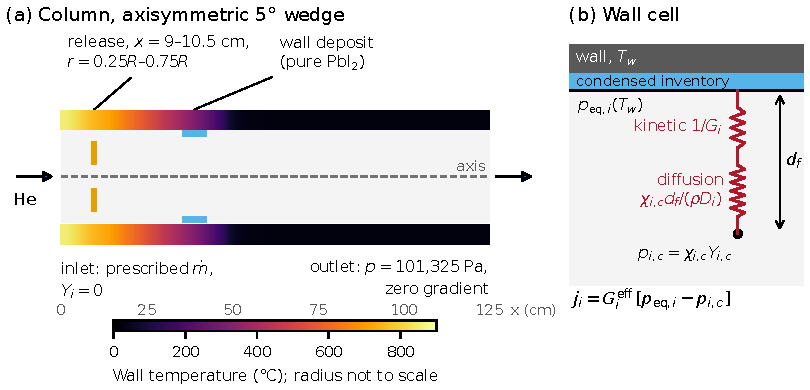
\includegraphics{experiment_schematic.pdf}
\caption{Computational geometry and prescribed source region. The
source is distributed over selected cells; the sketch does not show a
resolved boat surface. The model keeps the tube length and the
material-specific diameters, and the 5$^\circ$ wedge provides the
axisymmetric reduction.}
\label{fig:geometry}
\end{figure*}

The inlet flow rates are converted to helium mass flow assuming a
controller reference of 298.15 K and 101,325 Pa, which the supplied
paper does not specify. Full-column rates are
$2.727\times10^{-7}\units{kg\,s^{-1}}$ at 100 mL/min and
$1.227\times10^{-7}\units{kg\,s^{-1}}$ at 45 mL/min; a separate study
uses a 273.15 K reference. Helium follows the perfect-gas law with
constant heat capacity and Sutherland viscosity (supplementary
material, Sec.~S5). Steady laminar carriers are computed with
\texttt{rhoSimpleFoam} while the reconstructed temperature profile stays
prescribed. The converged face mass flux is corrected to discrete
continuity within $10^{-12}$ of the inlet flow (supplementary material,
Sec.~S2), which makes the frozen transport field conservative but is
not evidence that the velocity field has converged.

The boundary conditions are the same in all Liu et al.\ cases. At the
inlet the carrier enters with the prescribed mass flow at the local
wall temperature, and every reactive gas has a fixed mass fraction of
zero: clean helium enters, and the release is a volumetric source in
the source cells. At the outlet the static pressure is fixed at
101,325 Pa, an assumed value because neither experimental paper states
the column pressure, and all gases have zero normal gradient, so they
leave by advection. At the wall the transported gases have zero normal
gradient in the transport operator, and all wall exchange enters as the
face fluxes of \cref{sec:wall}. With the 101,325 Pa outlet pressure and
the baseline diffusivity, the Schmidt number is 2.0--11.3 between 400
and 1173 K, and the diameter-based P\'eclet number $\mathrm{Pe}=\mathrm{Re}\,\mathrm{Sc}$
is 5.9--17.4 at 100 mL/min and 2.6--7.8 at 45 mL/min. Axial diffusion
is therefore not negligible next to advection, and the fixed zero
inlet value permits a diffusive loss of vapor through the inlet; it is
included in the outward transport of the material ledger
(\cref{eq:balance}). The flow-stop cases replace both end conditions by
zero normal species flux (supplementary material, Sec.~S1).

\subsection{Transport regime}
\label{sec:regime}
With the full-column helium mass flow $\dot m$, the tube diameter $d$
and the Sutherland viscosity, $\mathrm{Re}=4\dot m/(\pi d\mu)$ is
1.5--3.0 for the 100 mL/min steel case and 0.7--1.3 for the 45 mL/min
cases between the source-furnace temperature of 1173 K and 400 K; the
carrier is laminar throughout. With the baseline diffusivity, the
radial diffusion time $R_t^2/D_i$ is 58 ms in steel and 63 ms in silica.
Placing the conductance of \cref{eq:hks} in series with diffusion over
the tube radius, as in \cref{eq:halfcell} with $d_f$ replaced by $R_t$
and $T_c=T_w$, defines a wall Damk\"ohler number
\begin{equation}
 \begin{aligned}
 \mathrm{Da}_i&=\frac{G_i\chi_iR_t}{\rho D_i}\\
 &=C_es_i\frac{2\alpha_i}{2-\alpha_i}
  \sqrt{\frac{RT_w}{2\pi M_i}}\,\frac{R_t}{D_i},
 \end{aligned}
 \label{eq:damkohler}
\end{equation}
where $R$ is the universal gas constant and $R_t$ is the tube radius. Because $\chi_i/\rho=RT_w/M_i$, it does not
depend on pressure. For
PbI$_2$ and BiI$_3$ between 400 and 1173 K, the baseline coefficients
give $\mathrm{Da}_i\approx1.4\times10^3$--$2.9\times10^3$, and the
tested accommodation coefficients $\alpha_i=0.1$ and 0.01 give about
76--150 and 7--15. This tube-scale estimate places the interfacial
resistance well below the radial diffusion resistance for
$\alpha_i=1$ and 0.1, and about an order of magnitude below it for
$\alpha_i=0.01$. It is a scaling estimate, not a substitute for the
resolved near-wall gradients of the calculations.
% TODO(review-B): Damkoehler sweep (running). Insert its result here: the
% computed response of the iodine profiles over the swept Da range, and
% whether it confirms the diffusion-limited reading of this paragraph and
% of Sec. 7.3. Do not change the PoF title before this is in.

Two omitted effects can be bounded with the same inputs, the digitized
wall profiles and the 101,325 Pa outlet pressure. The first is
buoyancy. Neither experimental paper states the column orientation. For
developed laminar flow with a linearly varying wall temperature, the
wall-to-bulk temperature difference is
$(11/192)\,U d^2|\mathrm{d}T_w/\mathrm{d}x|/a$, with $a$ the thermal
diffusivity of helium; it stays below 2.6 K. A Grashof number based
on the axial temperature change over one diameter,
$\mathrm{Gr}=g d^4|\mathrm{d}T_w/\mathrm{d}x|/(T\nu^2)$, stays below
2.2, and below 1.4 where the wall temperature lies between 400 and
750 K. Because Re is also of order one, the Richardson number
$\mathrm{Gr}/\mathrm{Re}^2$ reaches 0.15 (pure PbI$_2$) to 0.78
(silica) in that range, and about 1.2 in the steepest cold section of
the silica profile. Compositional buoyancy at the largest computed
trace mole fraction, $9.2\times10^{-5}$ evaluated with the molar mass
of BiI$_3$, gives $\mathrm{Gr}/\mathrm{Re}^2\le0.32$. Richardson numbers
of order 0.1--1 do not show that buoyancy is negligible: in a
horizontal column, buoyancy-driven secondary flow may be significant
locally, in particular in the steep cold sections where deposition
occurs. The frozen carrier does not represent it, and with the
orientation unknown its effect on the deposition profiles is an
unquantified limitation of the model. The second effect is thermal
(Soret) diffusion. Taking a thermal diffusion factor
$\alpha_T=1$ as a generous bound, the Soret drift velocity
$D_i\alpha_T|\mathrm{d}T_w/\mathrm{d}x|/T$ is at most 2.2\% of the
carrier velocity. The radial Soret flux, relative to a Fickian flux
$x_iD_i/R_t$ towards the wall, is at most $\alpha_T\Delta T_r/T\le0.7\%$,
with $\Delta T_r$ the wall-to-bulk difference above. Both are small
compared with the factor-of-two diffusivity variations examined in
\cref{sec:sensitivity}.

\subsection{Discretisation and coupling}
The transient species equations use implicit Euler time integration
and corrected Gauss linear diffusion. The production cases (the 15
baselines and four silica temperature-coordinate cases) use the bounded
OpenFOAM scheme \texttt{Gauss limitedLinear 1}
\cite{Jasak1996error,Sweby1984high} for advection on 41,472 cells. It
blends linear and upwind interpolation through a TVD-type flux limiter,
which reverts to upwinding near extrema and steep gradients. The 64
follow-up cases and the time-step comparisons keep the first-order
upwind advection of the original campaign on 18,432 cells, and the
follow-up sensitivities are always reported as differences from their
own upwind baselines on that mesh.
% TODO(review-A): production-scheme sensitivities (running). When they are
% complete, state here which follow-up sensitivities were repeated with
% limitedLinear on 41,472 cells and that Sec. 7.3 / Table VII report them.
The scheme and mesh study adds the van Leer limiter
\cite{vanLeer1974towards} (\texttt{Gauss vanLeer}) as a second bounded
scheme. All nine transported gases use the same advection scheme
within a case. The baseline time
step is 2 ms. Wall exchange is assembled implicitly with nonnegative
source and sink coefficients and shared inventory bounds. Configured
species correctors and active-bound guards reconcile the final gas
solution with the realized wall transfer. Gas re-speciation then
redistributes species under the local element constraints. The
sequence is first order in time; a conservative equilibrium projection
alone does not remove splitting or transport error. The baseline
configuration requests three species correctors with a $10^{-16}$
tolerance and up to eight bound guards with a $10^{-13}$ guard
tolerance; the effect of this stopping criterion is tested in
\cref{sec:conservation}.

Every gas has the baseline diffusivity $D_i=10^{-4}\units{m^2\,s^{-1}}$.
Three transport alternatives halve or double this value for all gases,
or replace only the PbI$_2$ coefficient with a temperature- and
pressure-dependent PbI$_2$--He estimate whose collision parameters are
themselves estimates (supplementary material, Sec.~S5). Accommodation
variations set $\alpha=0.1$ or 0.01 for the two reversible iodide pairs
and keep the baseline metal-channel coefficients.

\subsection{Completed case matrix}
The 15 baseline cases are Q1 for each available configuration, plus Q2
for the two LBE columns at $\beta\in\{0.001,0.01,0.1\}$ with two
thermodynamic branches. The second branch adds a constant 29 kJ/mol to
the standard Gibbs energy of BiI(g); it is a sensitivity surrogate, not
a second dataset. The 64 follow-up cases vary mesh and time step,
diffusivity, accommodation, source position, Q2 metal loading, flow
reference, silica temperature coordinate and a fixed-temperature flow
stop; they are a structured set of conditional comparisons, not a
factorial uncertainty study. Four further sets complete the evidence:
the \ProductionCases{} production re-runs (\cref{sec:verification}), a
scheme and mesh study of two cases up to 93,312 cells, three full-run
corrector checks, and ten runs of five single-species experiments of
Lobresco et al.\ \cite{Lobresco2026assessment} on two meshes
(\cref{sec:lobresco}). All Liu et al.\ calculations and the Lobresco
runs use the same solver executable, identified by its SHA-256 in the
saved reports. Table~S1 and Sec.~S1 of the supplementary material list
every case, its variation and its reference case.

\section{Numerical verification and resolution limits}
\label{sec:verification}
This section reports material conservation and solver diagnostics, then
the separate time-step and mesh comparisons, and finally two effects
that limit how precisely local profile features are resolved.

\subsection{Completion, material balance and solver diagnostics}
\label{sec:conservation}
All 15 runnable baseline cases, all 64 follow-up cases, the 19
production cases and the three full-run corrector cases completed and
passed their configured numerical acceptance checks; the scheme and
mesh runs completed with the same ledgers. This PASS
classification means only that the computation completed and passed
those checks; it is not an experimental-validation classification.
Element conservation is examined in two ways: through the solver
ledger and through an independently formed material residue. For
element $k$ the residue is
\begin{equation}
 \begin{aligned}
 R_k={}&N_k^{\rm gas}+N_k^{\rm wall}+N_k^{\rm sample}
     +N_k^{\rm net\,out}+N_k^{\rm removed}\\
     &-N_k^{\rm initial}-N_k^{\rm released},
 \end{aligned}
 \label{eq:balance}
\end{equation}
where $N_k$ are molar atom inventories and outward transport is signed.
The ledger also records the linear-solve defect and any clamping
correction separately. These terms explain bookkeeping closure, but
they are not inserted into $R_k$ when the raw material balance is
assessed.

All residues below are divided by the supplied material and taken as
the largest value over recorded steps and represented elements. The
largest raw residue is $\ProductionResidue$ for the 19 production cases
(41,472 cells, limited-linear advection) and $8.85\times10^{-13}$ for
the 60 source-driven follow-up cases; the 18,432-cell upwind baselines
had $5.97\times10^{-13}$. For the follow-up cases, the largest
accounted closure is $9.60\times10^{-16}$ and the largest recorded
solver defect is $8.64\times10^{-13}$; for the production cases they
are $1.12\times10^{-15}$ and $1.45\times10^{-12}$. The four
flow-stop cases keep their restart ledger and are excluded from this
summary of newly accumulated source material. These results support
conservation of the executed discrete model. They do not quantify
physical accuracy or discretisation error.

The baseline logs report no gas-equilibrium solver failures and a
maximum equilibrium element residue of $6.43\times10^{-16}$.
Input-validity and solver-success counters are distinct. At startup,
sign flags caused equilibrium to be skipped in up to 1,170 cells on
one step, and the maximum negative iodine diagnostic was
$1.14\times10^{-124}$ of supplied iodine. Matched five-step startup
replays identified extremely small leading-tail inventories at these
flags; no flagged cells remained at the final step. The calculations
should therefore not be described as free of negative trace values,
even though the reported amount is immaterial to the macroscopic
balance. The sum of the individual species mole-fraction maxima was at
most $9.19\times10^{-5}$. Because these maxima need not coincide, this
is an upper bound on the reactive trace loading, not a measured
mixture mole fraction at one location.

Some paired wall-coupling iterations did not meet the requested
$10^{-16}$ outer criterion. This is reported separately from
equilibrium failure, the final transport defect and the inventory-bound
checks. To test its effect, matched restarts of four representative
cases at 59 s compared three and eight correctors, and outer
tolerances of $10^{-16}$ and $10^{-14}$, over 20 time steps (40 ms).
The largest species-field change, scaled by its control maximum, was
below $3.6\times10^{-8}$, and the changes in new wall increments were
negligible. Three cases were then repeated over the full 60 s with
eight instead of three correctors (18,432 cells, upwind). The iodine
profiles of pure PbI$_2$ and of the steel Q2 case at 0.1\% saturation
change by $\IterPure\%$ and $\IterSteelLow\%$, that is, at round-off;
the steel case at 1\% saturation changes by \IterSteelHigh\%. With
eight correctors the largest outer initial residual is still
$2.4\times10^{-15}$--$4.4\times10^{-15}$, and nearly every step ends
at the corrector limit, as with three. The requested $10^{-16}$ lies
below the attainable residual floor, and the iteration error of the
reported profiles is negligible next to the time-step and spatial
errors below. No manufactured-solution test is presented.
\Cref{sec:lobresco} compares the model with published measurements
and published model results; it is not a code-to-code verification
with identical inputs.

\subsection{Separate time-step and mesh comparisons}
For profiles on the common 1 cm bins, let $a_b$ be the deposited
iodine atoms in bin $b$ for a comparison case and $a_b^0$ the
corresponding baseline inventory. We report the profile change
$E_{L1}$ and the total change $\Delta N_I$:
\begin{equation}
 E_{L1}=100\frac{\sum_b|a_b-a_b^0|}{\sum_b a_b^0},
 \qquad
 \Delta N_I=100\frac{\sum_b a_b-\sum_b a_b^0}{\sum_b a_b^0}.
 \label{eq:numeric-l1}
\end{equation}
Both measures retain changes in amount. The figures also show
normalised shape curves; these must not be confused with the
unnormalised profile change. Source, physical coefficients,
equilibrium engine and executable are fixed within each numerical
comparison.

\Cref{tab:numerical} separates time-step from mesh and scheme effects.
For successive mesh levels the reference $a_b^0$ is the finer level.
Reducing the time step from 2 to 1 ms on 18,432 cells changes the
iodine profile by \TimeMin--0.3228\%. With the upwind scheme of the
original campaign, the 18,432 to 41,472-cell differences of the four
follow-up cases are \MeshMin--\MeshMax\%, and the shifted-BiI steel
case changes by essentially the same amount on the first two
refinements (\SteelUpOne\% and \SteelUpTwo\%). Total deposited iodine
changes by less than 0.014\% from 18,432 to 41,472 cells, and the
centroid moves by at most 0.0652 cm. Integral quantities are thus
stable while local profile shapes still differ appreciably.
\begin{table*}[tb]
\centering
\caption{Iodine profile changes $E_{L1}$ (percent) between successive
mesh levels at 2 ms, relative to the finer level, for three advection
schemes, and the effect of halving the time step on 18,432 cells with
upwind advection. All steel cases are Q2; the shifted-BiI case uses
1\% metal saturation. The upwind levels of the two lower steel cases
are the follow-up cases of \cref{tab:study}. A dash marks a combination
that was not run.}
\label{tab:numerical}
\small\input{generated/numerical-table}
\end{table*}

\begin{figure*}[tb]
\centering
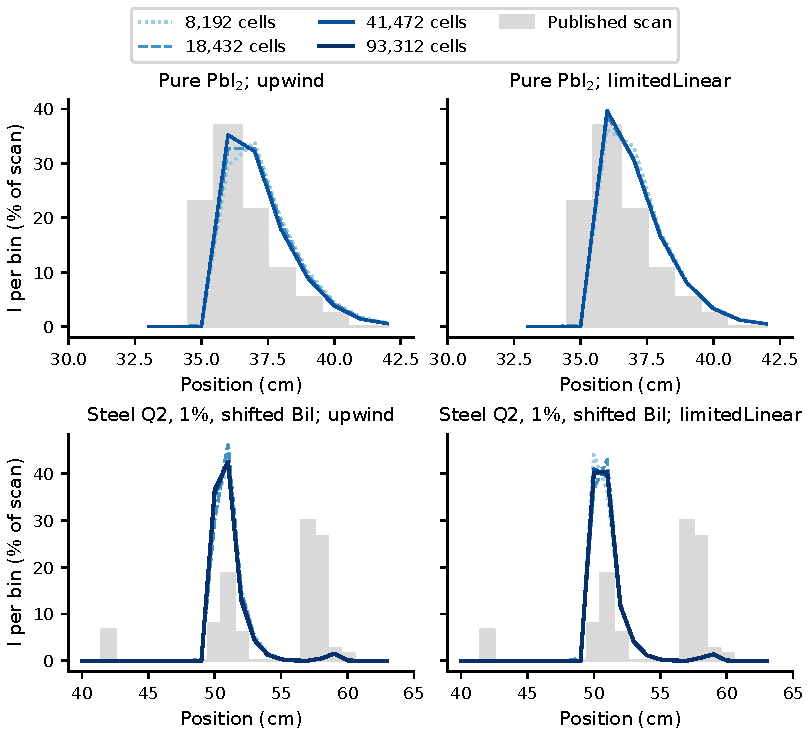
\includegraphics{refinement.pdf}
\caption{Mesh sequences of the iodine deposition profile for pure
PbI$_2$ (top) and the shifted-BiI steel case at 1\% metal saturation
(bottom), with first-order upwind (left) and limited-linear (right)
advection. Each curve is normalised over the common scanned interval
so that shapes can be compared; the unnormalised differences are given
in \cref{tab:numerical}. Grey histograms are the reconstructed
experimental iodine scans \cite{Liu2025chemical} and include any KI
contribution.}
\label{fig:refinement}
\end{figure*}

The scheme and mesh study (\cref{tab:numerical,fig:refinement})
addresses the shifted-BiI steel case directly. With the limited-linear
scheme its iodine profile changes by \SteelLLOne, \SteelLLTwo{} and
\SteelLLThree\% over the three refinements to 93,312 cells; with
upwind, by \SteelUpOne, \SteelUpTwo{} and \SteelUpThree\%. Pure
PbI$_2$ changes by \PureLLOne{} and \PureLLTwo\% with limited-linear,
against \PureUpOne{} and \PureUpTwo\% with upwind. The van Leer scheme
gives successive changes close to those of limited-linear and differs
from it by at most \VLSteelMax\% (steel) and \VLPureMax\% (pure
PbI$_2$) at equal mesh, and by \VLSteelThree\% and \VLPureThree\% on
41,472 cells. Between 41,472 and 93,312 cells, the 3 cm smoothed
profile of the steel case changes by \SteelSmoothThree\% and its total
deposit by \SteelTotalThree\%; over all four levels its centroid stays
within \SteelCentroidRange{} mm and the wall temperature at the PbI$_2$
centroid within \SteelCentroidTRange{} K.

Three-grid scalar checks follow the distinction between refinement
trends and an established asymptotic range
\cite{NASAGridConvergence,Roache1994perspective,Celik2008procedure}.
For the earlier upwind follow-up triplets, 17 of the 34 nontrivial or
zero-valued combinations of species, total, centroid and width are
oscillatory, four have nondecreasing differences, one is unresolved at
roundoff and 12 admit only conditional Richardson/GCI estimates. For
the limited-linear steel sequence, the iodine total, centroid and
width oscillate on both triplets, and the successive profile changes
give apparent orders of \SteelOrderOne{} and \SteelOrderTwo. These
orders are inconsistent, so no formal grid convergence index is
claimed. We quote the measured 41,472 to 93,312-cell change of
\SteelLLThree\% as the spatial uncertainty indicator of the production
profiles. If the last change were extrapolated at the last apparent
order, the 41,472-cell profile would lie about \SteelErrApparent\% from
the mesh limit; assuming second order, about \SteelErrSecond\%. These
are indicative estimates for one case, not confirmed uncertainty
bounds, and they do not establish mesh independence of local profile
shapes in other cases.

\subsection{Binned maxima and numerical diffusion}
A deposition maximum picked on a 1 cm grid is fragile when adjacent
bins have similar heights. In pure PbI$_2$ the 18,432-cell upwind
maximum is at 37 cm and 350.7\,$^\circ$C, while the 36 cm bin is only
about 0.05\% lower. On the 41,472-cell upwind mesh the maximum moves to
36 cm and 366.5\,$^\circ$C, although the centroid shifts by only
$-0.0585$ cm. With the production scheme (41,472 cells, limited-linear)
the binned maximum stays at 36 cm and 366.4--366.5\,$^\circ$C on all
three levels, and on 41,472 cells the 37 cm bin is 23\% lower, yet the maximum of the 3 cm
smoothed profile is at 37 cm and 350.5\,$^\circ$C, and the wall
temperature at the deposit centroid (37.11 cm) is 348.7\,$^\circ$C.
In the limited-linear steel sequence the PbI$_2$ maximum alternates
between two nearly equal bins, 50 and 51 cm (306.3, 288.1, 306.7 and
288.1\,$^\circ$C on the four levels), while the 3 cm smoothed maximum
stays at 51 cm and 288.0--288.1\,$^\circ$C and the centroid temperature
at 290.6--291.5\,$^\circ$C. In the upwind steel Q2 0.1\% case, the
dominant BiI$_3$ bin moves from 57 to 58 cm, and its reported
temperature changes from about 166.4 to 138.8\,$^\circ$C. A one-bin
switch can therefore change the peak temperature by nearly 28 K without
a comparable displacement of the profile as a whole. Peak temperature
alone is an insufficient convergence metric; \cref{tab:peaks} therefore
also reports the smoothed and centroid values.

First-order upwind advection, used in the original campaign and the
follow-up cases, smooths the profiles. The local one-dimensional
estimate $D_{\rm num}\simeq|u_x|\Delta x/2$ is comparable to or greater
than the prescribed $10^{-4}\units{m^2\,s^{-1}}$ diffusivity in parts of
the carriers. This is a Taylor-series screening estimate, not a
measured truncation error for the radial, variable-density coupled
problem, but the scheme study confirms its consequence. At equal mesh,
upwind differs from limited-linear by \UpLLOne, \UpLLTwo, \UpLLThree{}
and \UpLLFour\% for the steel case on the four levels and by
\PureUpLLMin--\PureUpLLMax\% for pure PbI$_2$, much more than the two
bounded schemes differ from each other. Upwind numerical diffusion is
therefore the dominant spatial error of the original campaign, and it
is why halving the time step could not establish convergence of
profile widths. Across the 19 production cases, the production profiles
differ from the 18,432-cell upwind profiles by 9.1--22.3\%. The
follow-up sensitivities of \cref{sec:sensitivity} remain upwind
differences on 18,432 cells, taken against baselines with the same
numerical error.

\subsection{Dependence on comparison-bin width}
\label{sec:bin-audit}
To distinguish sensitivity of the reported observable from a change in
the CFD mesh, the saved 1 cm iodine inventories of the original upwind campaign
were summed into groups
of two and four consecutive bins. Every possible integer-bin offset was
tested for each width, retaining partial end groups and the full deposited
inventory. No CFD field was recomputed and no sub-bin reconstruction was
introduced. \Cref{tab:bin-audit} gives the fine/medium inventory differences
for these coarser observables. Ranges reflect bin origin, not statistical
uncertainty.
\begin{table*}[tbp]
\centering
\caption{Original upwind fine/medium iodine inventory-profile differences
(percent, 41,472 versus 18,432 cells) after
aggregation of native bins. The 2 and 4 cm ranges cover all respective
integer-bin offsets. $W_1$ uses the original 1 cm bin centres and separately
normalised profiles; it measures redistribution distance, not position error
against the experiment.}
\label{tab:bin-audit}
\small\input{generated/resolution-audit-table}
\end{table*}

For the shifted-BiI case, a 4 cm comparison gives differences from
0.52\% to 10.02\% depending on the grouping origin. Thus a favourable
aggregation can hide a substantial local difference. Summing signed
bin differences before taking their absolute values necessarily allows
cancellation; reduced aggregated L1 is not additional convergence evidence.
The largest difference remains appreciable even at 4 cm resolution.

As a complementary position-sensitive measure, let $p_b$ and $q_b$ be
the fine and medium iodine inventories normalised separately over the
whole column, and $x_b$ their common native bin centres. The
one-dimensional transport distance for these discrete distributions is
\begin{equation}
 W_1=\sum_{b=1}^{B-1}\left|\sum_{j=1}^{b}(p_j-q_j)\right|
                  (x_{b+1}-x_b).
 \label{eq:binned-wasserstein}
\end{equation}
It is the minimum mean distance needed to redistribute one normalised
binned inventory into the other. Values of 0.0115--0.0711 cm indicate
small average spatial redistribution between the two tested meshes,
despite larger local L1 differences. This is a distance between computed
binned profiles, not a bound on continuum error or evidence that the
experimental position uncertainty has been resolved.

\section{Conditional comparison with deposition measurements}
\label{sec:comparison}
This section compares the calculations, mainly the original Q1 cases,
with the reconstructed deposition scans. The comparisons are
conditional on the reconstructed inputs and assumptions of
\cref{sec:experiments,sec:model}; they are not independent validation.

\subsection{Comparison measures}
The primary comparison uses reconstructed relative iodine yields per
1 cm bin. Let $e_b$ be the experimental percentage and let
\begin{equation}
 m_b=(100-y_{\rm KI})\frac{a_b}{\sum_{\rm full\ column}a_b}
 \label{eq:yield}
\end{equation}
be the modelled percentage, where the stated excluded KI yield is
$y_{\rm KI}=0$, 6.6 or 7.0. Over the common scanned bins $\mathcal B$,
we report the raw discrepancy
\begin{equation}
 L_{\rm raw}=\sum_{b\in\mathcal B}|m_b-e_b|
 \quad\text{(percentage points)}.
 \label{eq:raw-l1}
\end{equation}
This measure keeps the experimental digitisation sum and the model's
explicit KI exclusion. It is neither an absolute deposited-mass error
nor a percentage relative to an experimental uncertainty.

A secondary shape diagnostic normalises both profiles over
$\mathcal B$, $\widehat m_b=m_b/\sum_{\mathcal B}m_b$ and
$\widehat e_b=e_b/\sum_{\mathcal B}e_b$, and computes the overlap
\begin{equation}
 O=100\sum_{b\in\mathcal B}\min(\widehat m_b,\widehat e_b).
 \label{eq:overlap}
\end{equation}
The overlap $O$ is conditional on the common scanned range and discards
differences in capture and total yield. The experimental normalisation
still contains KI. $O$ is a descriptive shape measure, not a validation
probability or a fitted goodness-of-fit statistic.

\subsection{Q1 peaks and complete profiles}
\Cref{tab:peaks} compares the five available Q1 iodide maxima with the
printed peak temperatures. All calculated peak temperatures lie within
the stated temperature ranges. Pure PbI$_2$ lies near the
low-temperature edge of its range, and its binned maximum moves under
refinement (\cref{sec:verification}). Steel LBE places both iodide
maxima at the measured positions, whereas silica LBE places the
PbI$_2$ and BiI$_3$ maxima 5 and 4 cm downstream, respectively.
Agreement with a printed temperature is therefore not sufficient to
establish the correct spatial location.
\begin{table}[tb]
\centering
\caption{Q1 iodide maxima on the original 18,432-cell mesh, compared
with the published peaks. Positions are in cm and temperatures in
$^\circ$C. Experimental temperature ranges are those printed by Liu et
al.\ \cite{Liu2025chemical}; they are not statistical confidence
intervals for model error.}
\label{tab:peaks}
\small\input{generated/peaks-table}
\end{table}

\Cref{fig:baseline} shows the complete profiles. The raw discrepancies
$L_{\rm raw}$ are 53.90, 53.45 and 181.84 percentage points for pure
PbI$_2$, steel LBE and silica LBE, and the corresponding normalised
overlaps are 72.93\%, 71.88\% and 7.20\%. The silica case therefore
has a large profile discrepancy even though both printed temperature
ranges contain its calculated maxima.
\begin{figure*}[tb]
\centering
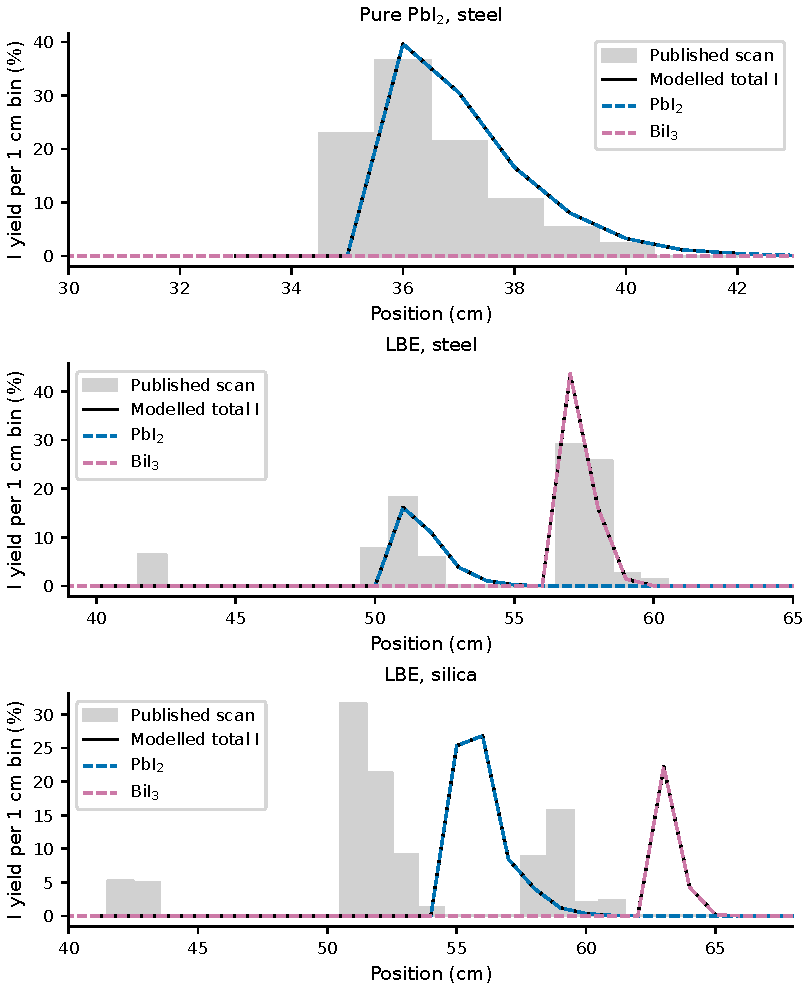
\includegraphics[width=\textwidth]{baseline_profiles.pdf}
\caption{Original Q1 iodine profiles compared with the digitised
published scans (grey histograms) \cite{Liu2025chemical}. Solid black
lines are total modelled wall iodine; dashed lines show its two iodide
contributions. Model totals are normalised to 100\%, 93.4\% and 93.0\%
for pure PbI$_2$, steel LBE and silica LBE, respectively, to expose the
omitted KI yield; experimental bars keep their digitised values.}
\label{fig:baseline}
\end{figure*}

The Q1 steel BiI$_3$ share of deposited iodide iodine is 65.34\%, close
to the measured iodide-only share of $61.3/(61.3+32.1)=65.63\%$.
For silica the corresponding values are 28.68\% and
$27/(27+66)=29.03\%$. These agreements are substantially conditioned
by the source masses, which were inferred from the same deposits. They
cannot serve as independent validation of gas speciation or LBE
release. Similarly, the source-driven calculations capture
91.27--98.20\% of the supplied iodine on the wall by 60 s. This does
not establish the experimental three-hour capture, because the
remaining inventory, the release history and post-release cooling are
different questions.

\section{Input sensitivity and interpretation}
\label{sec:sensitivity}
This section examines how source loading, BiI thermodynamic data, the
silica temperature coordinate, and transport, kinetic and flow inputs
change the computed deposits.

\subsection{Source loading and thermodynamic input}
The Q2 cases expose a sensitivity that is hidden when the iodide split
is prescribed. \Cref{fig:thermo} shows the BiI$_3$ share of deposited
iodide iodine,
\begin{equation}
 f_{\rm BiI_3}=
 \frac{3N^{\rm wall}_{\rm BiI_3}}
 {2N^{\rm wall}_{\rm PbI_2}+3N^{\rm wall}_{\rm BiI_3}},
 \label{eq:split}
\end{equation}
which counts only the iodine in the two modelled iodides and therefore
differs from the BiI$_3$ fraction of all experimental iodine, which also
contains KI.

At 1\% metal saturation on the production steel mesh, the baseline
thermodynamics give $f_{\rm BiI_3}=94.58\%$ (94.57\% with upwind
advection). Raising the BiI(g) standard Gibbs energy by 29 kJ/mol,
consistently in the formation and reactive-wall constants, gives 2.01\%
(2.00\%). A constant shift of this size scales the formation constant by
$\exp[-29{,}000/(RT)]$, approximately 0.051 at 1173 K and 0.00093 at
500 K. An independent integration of the saved species profiles of the
original upwind campaign gives 94.532--94.569\% and 1.922--2.004\% over
three meshes and the half-step run, a separation of 92.555--92.619
percentage points at every matched resolution. The response is
therefore not numerical noise. What it measures is the importance of
the BiI thermodynamic input for the predicted iodide partition: a
single, arbitrarily sized perturbation moves the partition almost from
one iodide to the other. The shift is not an estimate of the
uncertainty of the BiI data, the two branches do not bound an
uncertainty interval, and the comparison with the measured split is not
a basis for selecting either dataset.

Source loading also matters. With baseline thermodynamics, the steel
BiI$_3$ share at 0.2\%, 0.316\% and 0.562\% metal saturation
(follow-up cases, 18,432 cells, upwind) is 52.50\%, 70.58\% and
94.56\%; the shifted branch gives 47.66\%, 37.43\% and 15.88\%. The
low-loading trend is not universally monotonic. The steel 0.1\% case
with baseline thermodynamics gives 56.48\% and an 80.66\% scan overlap
(56.47\% and 81.10\% on the 18,432-cell upwind mesh), a useful
diagnostic comparison but not an identified physical saturation. The
published deposits alone cannot separate source loading, thermodynamic
data and omitted chemistry; choosing a branch because it best matches
one scan would be a calibration.

\begin{figure*}[tb]
\centering
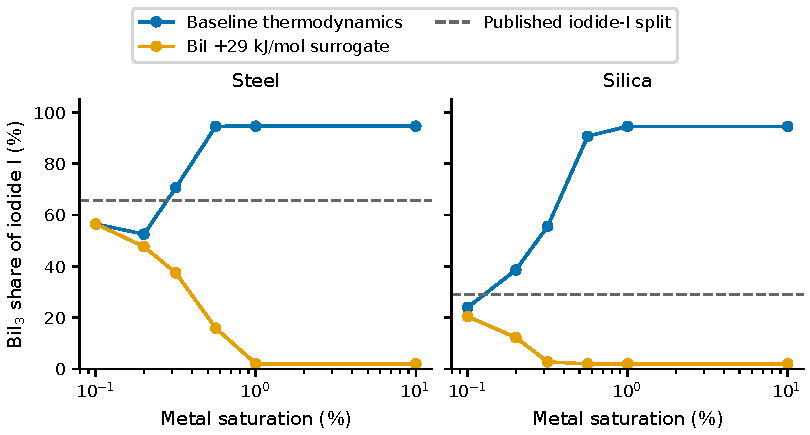
\includegraphics{source_thermodynamics.pdf}
\caption{BiI$_3$ share of deposited iodide iodine (\cref{eq:split})
against source loading for the baseline and the $+29$ kJ/mol BiI
thermodynamics, for steel and silica LBE. Symbols denote completed Q2
cases; segments only connect those points. Dashed grey lines show the
published BiI$_3$ share after excluding KI \cite{Liu2025chemical}.
The $+29$ kJ/mol branch is a surrogate perturbation, not a second
qualified thermodynamic dataset.}
\label{fig:thermo}
\end{figure*}

\subsection{Silica temperature-coordinate inconsistency}
\label{sec:silica}
In the silica experiment the published peak labels do not match the
published temperature curve. The scan places the PbI$_2$ and BiI$_3$
maxima at 51 and 59 cm, labelled 306$\pm$24 and 127$\pm$39\,$^\circ$C.
At those positions the digitized temperature curve gives approximately
369 and 235\,$^\circ$C, 63 and 108 K above the labels; on the same curve,
306 and 127\,$^\circ$C occur at 55.096 and 63.653 cm. The discrepancy
exceeds the nominal raster temperature resolution, so the published
inputs contain a temperature-coordinate inconsistency; they do not say
which measurement, annotation or registration is in error.

Two diagnostic mappings shift only the silica temperature curve
upstream, by 4.096 or 4.653 cm, so that one of these curve crossings
aligns with the corresponding labelled position:
$T_\delta(x)=T_0(x+\delta)$ for $\delta>0$, with
$\Delta x_T=-\delta$. The iodine scan stays fixed. The shifts are
derived from the published curve and labels, not optimised against the
CFD profiles.

\Cref{tab:alignment,fig:alignment} show that the shifts move the Q1
maxima from 56/63 cm to 51/59 or 51/58 cm and raise the normalized
overlap from 6.13\% to 77.80\% or 73.26\%. The low-loading Q2 variants
place the maxima at 51/59 or 51/58 cm, with overlaps of 77.88\% and
75.54\%. On the 18,432-cell upwind mesh the order of the two shifts was
the opposite (75.29\% and 81.00\% for Q1; 79.16\% and 83.33\% for Q2),
so the overlap does not rank the two hypotheses robustly. The two shifts
also give different peak temperatures, and no single mapping reconciles
both labels. The shifted low-loading Q2 cases keep a BiI$_3$ share near
23.97\%, about five percentage points below the published iodide-only
split, so correct peak positions do not ensure the correct partition.

These results demonstrate the inconsistency and show that a plausible
coordinate change has a larger effect on the computed agreement than
the tested source-position or time-step changes. They do not resolve
the inconsistency: both shifts use labels from the same experiment,
neither is confirmed, and the improved agreement is conditional on an
unconfirmed hypothesis. Resolving it requires the original thermocouple
profile and its coordinate registration.
\begin{table}[tb]
\centering
\caption{Silica temperature-coordinate hypotheses: computed peak
positions and agreement with the fixed experimental scan for the
original and two shifted temperature curves. Shifts and peak positions
are in cm; raw L1 ($L_{\rm raw}$) is in percentage points and overlap
in percent. Q2 uses baseline thermodynamics and 0.1\% metal
saturation.}
\label{tab:alignment}
\small\input{generated/alignment-table}
\end{table}
\begin{figure*}[tb]
\centering
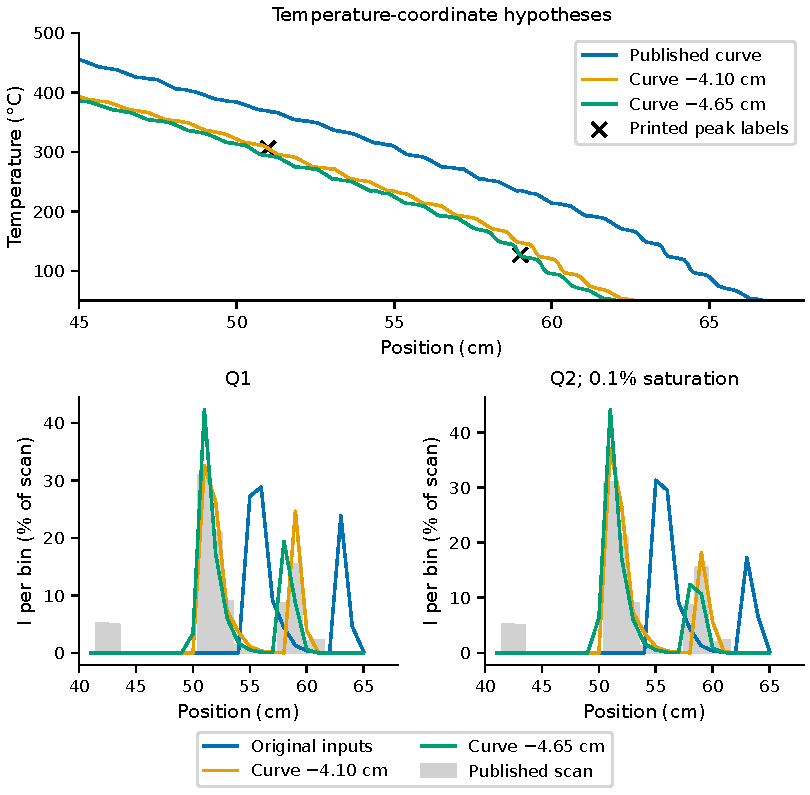
\includegraphics{silica_alignment.pdf}
\caption{Input-derived silica mappings and their consequences.
Top: the original reconstructed temperature curve, the two shifts and
the printed peak labels. Bottom: common-scan-normalized iodine
profiles for Q1 and low-loading Q2. The improved agreement is
conditional on an unconfirmed coordinate hypothesis. Published data
are adapted from Liu et al.\ \cite{Liu2025chemical}.}
\label{fig:alignment}
\end{figure*}

\subsection{Transport, kinetics, flow reference and flow stop}
\label{sec:transport-sensitivity}
\Cref{tab:sensitivity} reports, for each tested category, the range of
iodine profile changes $E_{L1}$ (\cref{eq:numeric-l1}) from the
designated baseline. These are responses to finite hypothetical
changes, not statistical confidence limits. The source-loading row uses
its 1\% reference case. The temperature-coordinate row measures changes
from the original silica input and can approach 200\% when the profile
supports move apart.
\begin{table}[tb]
\centering
\caption{Range of the baseline-relative iodine profile change $E_{L1}$
(percent) within each completed sensitivity category. The flow-stop row
compares 80 s inventories with their 60 s restart state; the other rows
compare 60 s inventories. The silica temperature-coordinate row uses
the production cases (41,472 cells, limited-linear advection); all
other rows are upwind follow-up cases on 18,432 cells compared with
their own upwind baselines; \cref{tab:production-sensitivity} repeats
the diffusivity and accommodation rows with the production scheme for
two cases. Case counts and variations are listed in Table~S1 of the
supplementary material.}
\label{tab:sensitivity}
\small\input{generated/sensitivity-table}
\end{table}
\begin{table}[tb]
\centering
\caption{Diffusivity and accommodation variations with the production
scheme (LL: limited-linear, 41,472 cells) and with upwind on 18,432
cells, each relative to its own baseline: iodine profile change
$E_{L1}$ (percent) and centroid shift $\Delta x_c$ (cm). Steel Q2 uses
baseline thermodynamics. Total deposits change by at most
\PSTotalMax\% and the BiI$_3$ share of iodide iodine by at most
\PSShareMax{} percentage points.}
\label{tab:production-sensitivity}
\small\input{generated/production-sensitivity-table}
\end{table}

Diffusion alternatives change profiles by up to 14.20\%. A 273.15 K flow
reference raises the inferred helium mass flow by 9.15\% relative to
298.15 K and changes profiles by up to 10.93\%. Iodide accommodation
changes give up to 4.21\%, whereas moving the prescribed source region
by $\pm1.5$ cm gives at most 0.19\%, a statement about the empty-tube
source model that cannot rule out an effect of a real boat on the flow.
Fig.~S1 of the supplementary material shows the maxima. They are differences between
upwind cases on the 18,432-cell mesh, which itself differs from the
production scheme by 12--14\% for the two cases of the scheme study
(\cref{sec:verification}). For the diffusivity and accommodation
variations, \cref{tab:production-sensitivity} shows how much of this
survives the scheme change. With the production scheme, $\alpha=0.1$
changes the iodine profile by \PSAlphaOneMin--\PSAlphaOneMax\% and
$\alpha=0.01$ by \PSAlphaTwoMin--\PSAlphaTwoMax\%, against
\PSDMin--\PSDMax\% for halving or doubling $D$; the pure PbI$_2$
responses are slightly larger than with upwind and nearly symmetric in
$D$. The steel response to $D$ is not: halving $D$ changes the iodine
profile by only \PSSteelHalf\% (upwind \PSSteelHalfUp\%), because the
BiI$_3$ profile, which carries most of the iodine, barely moves
(\PSSteelHalfBiI\% against \PSSteelHalfBiIUp\%), whereas doubling $D$
gives \PSSteelDouble\% (upwind \PSSteelDoubleUp\%). The diffusivity
response is therefore case-dependent and not linear in $D$, and in the
steel case $\alpha=0.01$ changes the profile more than halving $D$. The
other categories of \cref{tab:sensitivity} have upwind differences
only, so effects of comparable size there are not ranked precisely.
In both production-scheme cases, $\alpha=0.1$ changes the profile far
less than either diffusivity change. Together with the tube-scale
Damk\"ohler numbers of \cref{sec:regime} and the channel sweep of
\cref{fig:damkohler}, which places $\alpha=1$ and 0.1 on the
diffusion-limited plateau and $\alpha=0.01$ at its edge, this indicates
that radial diffusion, not interfacial kinetics, limits the wall
exchange in these columns; the wall temperature acts mainly through the
equilibrium pressure.

The four fixed-temperature flow-stop cases change the deposited iodine
profiles by 1.10--4.63\% over 20 s, with centroid shifts of at most
0.0422 cm. Residual gas can therefore alter wall inventories after
release stops, but because these runs neither cool the column nor flush
it, they do not predict the end-of-experiment redistribution.

\section{Discussion: implications for predictive modelling}
\label{sec:discussion}
\subsection{Conservation, resolution and experimental agreement}
The results separate three requirements that a deposition calculation
must satisfy. Element balance tests the consistency of the discrete
transport--equilibrium--wall coupling. Resolution studies test how much
the computed observables depend on numerical choices. Experimental
comparison tests the combined consequences of that numerical model,
its physical assumptions and its input data. Passing the first test
does not establish the other two.

This distinction is consequential here. The raw material residues are
small, but the original upwind fine/medium profile differences are
2.06--10.58\%.
Meanwhile, total deposition changes by less than 0.014\% under the same
refinement. An integral balance can therefore appear stable while the
spatial distribution remains sensitive. A binned peak introduces an
additional loss of information: nearly equal neighbouring bins can
exchange rank and produce a large change in the reported peak
temperature. Profile differences, centroids and deposited amounts
should accompany peak comparisons when assessing this model.
The production scheme and mesh study reduces the most sensitive
limited-linear profile change to \SteelLLThree\% between 41,472 and
93,312 cells, without a consistent apparent order.
The saved-profile aggregation check in \cref{sec:bin-audit} strengthens
this distinction: wider bins can suppress the apparent mesh difference,
but the result depends strongly on their origin. Conversely, the small
binned transport distances support stability of broad deposition location
between the tested meshes without qualifying local peak heights.

The physical-input variations also need to be interpreted against this
resolution evidence. Their ranges are finite responses over selected
cases, not components of a probabilistic uncertainty budget. They cannot
be added in quadrature or used to infer a universal parameter ranking.
The refined BiI perturbation retains a large change in iodide partition,
whereas several transport and accommodation responses are comparable
in magnitude to the unresolved spatial differences. The latter require
further numerical qualification before small physical effects can be
distinguished reliably.

\subsection{What the experimental comparisons can identify}
The source constructions expose a limitation of inferring release
chemistry from final deposits. Q1 uses deposit-derived compound masses
for LBE, so agreement in the iodide split partly reflects information
already supplied to the calculation. Q2 allows the split to emerge,
but combines a deposit-derived iodine loading with an unmeasured metal
saturation. The response to BiI thermodynamics then shows that the
same observed split may constrain several coupled assumptions rather
than identify a unique source or thermodynamic description.

The silica results reveal a separate ambiguity. Both the printed peak
temperatures and the digitised spatial scan appear plausible when
considered individually, yet they disagree through the reconstructed
temperature-coordinate mapping. The two diagnostic shifts substantially
improve the profiles without resolving which mapping is physically
correct; their overlap ranking reverses between upwind and limited-linear
advection. Moreover, these shifts use labels from the same experiment
being compared. Although they were not fitted to CFD output, their
improved agreement is still not an independent validation test.

The untuned single-species comparison with Lobresco et al.\
\cite{Lobresco2026assessment} supplies an additional experimental test:
the onset-temperature RMS deviation is \LobRMS{} K, but the computed
peaks lie \LobShiftMin--\LobShiftMax{} cm upstream and the shutdown
transient and non-dilute source region remain unrepresented. It strengthens
the evidence for the transport and wall law within those limits.

The practical contribution is therefore a framework for testing explicit
input hypotheses while retaining conservation and exposing profile
discrepancies. The present data do not uniquely separate release,
thermodynamic, coordinate and omitted-chemistry effects. Fitting an
interfacial coefficient to a single peak under these conditions could
compensate for an error elsewhere in the model.

\subsection{Evidence needed to extend the present scope}
The scheme and mesh study now extends the shifted-BiI steel branch to
93,312 cells with bounded advection, and full-duration corrector checks
are available for three cases. Spatial qualification still needs to extend
beyond that one refined branch and include cases with competing binned
maxima. Full profiles and integral observables should both be assessed.
The full-duration shifted-BiI corrector comparison remains unreported.

On the experimental side, the most direct constraints would be the
original thermocouple and scan coordinates, controller reference
conditions and an independently measured release history. Qualified
BiI thermodynamics and the provenance of the constructed condensed
records are also needed before selecting a thermochemical branch on
physical grounds. These requirements address specific ambiguities
demonstrated by the completed cases.

Finally, comparison with post-experiment deposits requires the release
and cooling protocol to be represented or its effect independently
bounded. The current 60 s calculations preserve the assumed three-hour
mean source rate, while the flow-stop restarts retain the original
temperature field. Neither calculation supplies the missing history.
The role of potassium chemistry, substrate reactions, finite gas
kinetics and boat obstruction remains outside the evidence presented
here and cannot be inferred from the present sensitivity ranges.

\section{Conclusions}
\label{sec:conclusions}
We have applied a conservative finite-volume treatment of nine
Pb--Bi--I gases and four shared condensed wall inventories in 15
baseline and 64 follow-up cases, 19 production re-runs and a scheme,
mesh and iteration study. The columns are treated as laminar
helium flows ($\mathrm{Re}\approx0.7$--3) in tubes with a steep axial
wall-temperature gradient, where axial advection, radial diffusion to
the wall and a reversible interfacial exchange law together set the
deposition profile. The reported calculations use a
specialised ideal-gas equilibrium kernel, a prescribed helium carrier
and reversible iodide wall exchange with half-cell diffusion
resistance. Material bookkeeping is tight: the worst raw element
residue is $8.85\times10^{-13}$ of supplied material in the follow-up
cases and $\ProductionResidue$ in the production cases. Conservation
is a numerical property of this model; it is not evidence that all
physical pathways are represented. Within the model, radial diffusion
rather than interfacial kinetics limits the wall exchange: the wall
Damk\"ohler number is large, and the profiles respond far more to the
diffusivity than to the accommodation coefficient.

Integral results are much less sensitive to resolution than local
profiles. Halving the time step changes iodine profiles by at most
\TimeMax\%, and eight instead of three species correctors over a full
run by at most \IterSteelHigh\%. The spatial error is larger and is
dominated by the numerical diffusion of the first-order upwind scheme
of the original campaign: at equal mesh it differs from the
limited-linear scheme by \UpLLFour--\UpLLOne\% in the most sensitive
case, whereas two bounded schemes differ by at most \VLSteelMax\%. With
limited-linear advection that case changes by \SteelLLThree\% between
41,472 and 93,312 cells, its total deposit by \SteelTotalThree\% and
its centroid by less than 1 mm, but the apparent orders are
inconsistent, so we quote this change rather than a formal grid
convergence index. The production cases therefore use limited-linear
advection on 41,472 cells, while the follow-up sensitivities remain
upwind differences on 18,432 cells. Closely competing 1 cm bins can make
a reported peak temperature switch by tens of kelvin under refinement,
so peaks are reported with their 3 cm smoothed maximum and centroid
temperature as well.

Thermodynamic and source assumptions substantially affect the computed
iodide partition. In the refined steel case, a $+29$ kJ/mol surrogate
shift of the BiI gas Gibbs energy changes the BiI$_3$ iodine share from
94.58\% to 2.01\% (94.57\% to 2.00\% with upwind advection on
18,432 cells). This sensitivity survives refinement, but it does
not determine which thermodynamic branch represents the experiment.
Q1 agreement is conditioned on inferred deposit masses, and Q2 keeps a
deposit-derived iodine source and an unmeasured metal saturation.

For silica, temperature-coordinate shifts derived from the published
inputs reduce the original 4--5 cm position discrepancies to 0--1 cm.
This identifies coordinate registration as a consequential
uncertainty, but it does not establish a corrected experimental
dataset, and the ranking of the two shifts by profile overlap reverses
between the upwind and limited-linear schemes. The supplied paper resolves neither that registration nor the
flow-reference conditions.

On five independent single-species PbI$_2$ experiments of Lobresco et
al., the same wall law without any tuning gives deposition-onset
temperatures with an RMS deviation of \LobRMS{} K, against
\LobRMSTemp{} and \LobRMSVap{} K for the two models of that study,
although the computed deposits lie \LobShiftMin--\LobShiftMax{} cm
upstream of the measured peaks and the flow-stop transient and the
non-dilute source region are not represented.

The present evidence supports a methods and input-sensitivity study.
Independent predictive validation would require better-constrained
source and thermodynamic inputs, consistent experimental coordinates,
tabulated wall temperatures, spatially qualified profile calculations
for more than one case and a treatment of the release and cooling
protocol. The completed cases show where
this additional evidence is needed, without hiding the original profile
discrepancies.


% IJHMT end matter (Elsevier declarations, data statement, supplement
% note), shared by both IJHMT wrappers.  Needs \confirm{}.
\section*{CRediT authorship contribution statement}
\textbf{Jan Kren}: \confirm{CRediT roles}.
\textbf{Bojan Ni\v{c}eno}: \confirm{CRediT roles}.

\section*{Declaration of competing interest}
\confirm{The authors declare that they have no known competing financial
interests or personal relationships that could have appeared to influence
the work reported in this paper.}

\section*{Declaration of generative AI and AI-assisted technologies in the
writing process}
\confirm{whether such tools were used and, if so, Elsevier's statement:
``During the preparation of this work the authors used [tool] in order to
[reason]. After using this tool, the authors reviewed and edited the
content as needed and take full responsibility for the content of the
publication.'' Remove this section if no such tool was used.}

\section*{Acknowledgements}
\confirm{acknowledgements and the funding statement with grant numbers.
The funding statements of an earlier draft were removed until the authors
confirm that they apply to this work.}

\section*{Data availability}
% Data availability statement shared by the journal builds (pof, ijhmt).
% Needs \confirm{} from the including file.
The solver, the benchmark preparation scripts and the data that support
the findings of this study are openly available in the LESTO repository
at \url{https://github.com/JanKren/LESTO},
\confirm{archived release or DOI, and that the branch holding these
files is public}. These files comprise the completed baseline,
follow-up, production, scheme and mesh, and iteration-check metrics,
the Graetz--Robin verification records, saved axial profiles,
generated tables,
figure-generation code and SHA-256 provenance records. The experimental
curves were digitised from Liu et al.\ \cite{Liu2025chemical}; they
reconstruct published figures, are not author-supplied measurements,
and are adapted under the source paper's CC BY 4.0 licence. The
measured profiles, wall temperatures and model curves of Lobresco et
al.\ \cite{Lobresco2026assessment} were digitised in the same way and
are adapted under that paper's CC BY 4.0 licence; the case set-up and
final profiles of our comparison runs are included. Some
thermodynamic coefficient files are external inputs that are not
redistributed; their local identifiers and the provenance of the derived
tables are recorded with the benchmark. Reproducing the CFD calculations
from the coefficients requires access to those inputs, whereas
regenerating the figures from the saved results does not.


\appendix
\section*{Supplementary material}
Supplementary material associated with this article (case inventory,
detailed material-ledger and solver diagnostics, scalar mesh checks of
the upwind campaign, comparison-bin-width analysis, property and
thermodynamic records, and the complete Graetz--Robin verification table)
is provided as a separate file.


\bibliographystyle{unsrtnat}
\bibliography{../references}
\end{document}
